\documentclass[tikz,border=8pt,multi=tikzpicture]{standalone}
\usepackage{amsmath}
\usepackage{xcolor}
\usetikzlibrary{arrows.meta, calc}

\definecolor{mainblue}{HTML}{001158}
\definecolor{accent}{HTML}{8592bc}
\definecolor{lightaccent}{HTML}{e7e9f2}

\tikzset{
  force/.style={-{Stealth[length=3mm]}, line width=1.2pt, color=mainblue},
  dim/.style={-{Stealth[length=2mm]}, line width=0.7pt, color=accent},
  moment/.style={-{Stealth[length=2.5mm]}, line width=1.2pt, color=mainblue},
  every node/.append style={font=\sffamily}
}

\begin{document}

% ---------- Concept sketch: general (non-concurrent) force system ----------
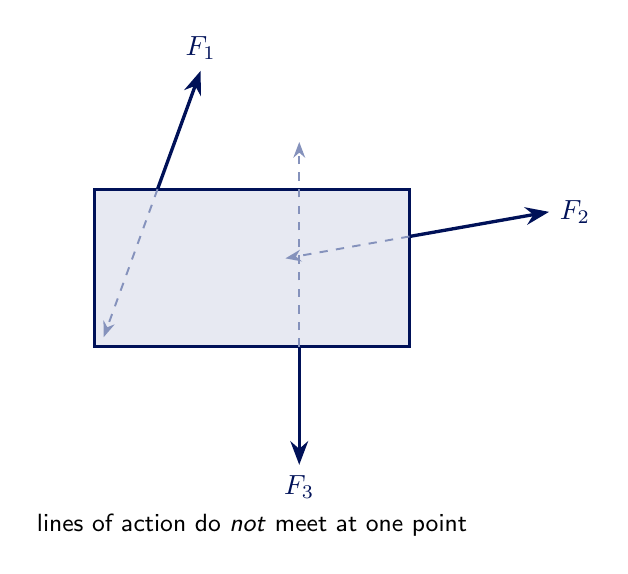
\begin{tikzpicture}
\fill[lightaccent, draw=mainblue, line width=1pt] (0,0) rectangle (4,2);
\draw[force] (0.8,2) -- ++(70:1.6) node[above] {$F_1$};
\draw[dim, dashed] (0.8,2) -- ++(250:2.0);
\draw[force] (4,1.4) -- ++(10:1.8) node[right] {$F_2$};
\draw[dim, dashed] (4,1.4) -- ++(190:1.6);
\draw[force] (2.6,0) -- ++(-90:1.5) node[below] {$F_3$};
\draw[dim, dashed] (2.6,0) -- ++(90:2.6);
\node[below] at (2,-2.0) {\small lines of action do \emph{not} meet at one point};
\end{tikzpicture}

% ---------- Exercise 2.1: two parallel forces on a beam ----------
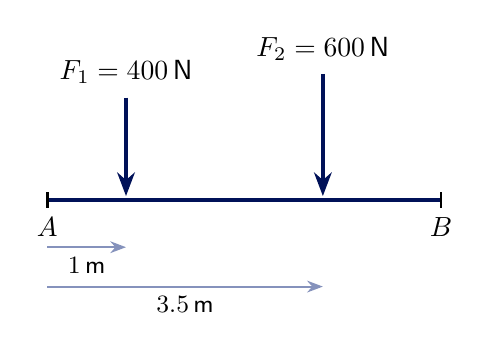
\begin{tikzpicture}
\draw[line width=1.5pt, mainblue] (0,0) -- (5,0);
\foreach \x in {0,5} {\draw[line width=1pt] (\x,-0.1) -- (\x,0.1);}
\node[below] at (0,-0.1) {$A$};
\node[below] at (5,-0.1) {$B$};
\draw[force] (1,1.3) -- (1,0.05) node[midway, right=2pt] {};
\node[above] at (1,1.35) {$F_1=400\,\text{N}$};
\draw[force] (3.5,1.6) -- (3.5,0.05);
\node[above] at (3.5,1.65) {$F_2=600\,\text{N}$};
\draw[dim] (0,-0.6) -- (1,-0.6);
\node[below] at (0.5,-0.6) {\small $1\,\text{m}$};
\draw[dim] (0,-1.1) -- (3.5,-1.1);
\node[below] at (1.75,-1.1) {\small $3.5\,\text{m}$};
\end{tikzpicture}

% ---------- Exercise 2.2: force at an offset point, equivalent system at O ----------
\begin{tikzpicture}
\draw[-{Stealth[length=2mm]}, line width=0.6pt, color=black!45] (-0.5,0) -- (4,0) node[right] {$x$};
\draw[-{Stealth[length=2mm]}, line width=0.6pt, color=black!45] (0,-0.5) -- (0,3) node[above] {$y$};
\fill[mainblue] (0,0) circle (2pt);
\node[below left] at (0,0) {$O$};
\fill[mainblue] (3,2) circle (2pt);
\node[above left] at (2.9,2.1) {$B\,(3,2)$};
\draw[dim, dashed] (3,0) -- (3,2) -- (0,2);
\draw[force] (3,2) -- ++(30:1.8) node[above right] {$F=500\,\text{N}$};
\draw[dim] (4.0,2) arc (0:30:1.0);
\node at (4.15,2.35) {\small $30^\circ$};
\end{tikzpicture}

% ---------- Exercise 2.3: bar pinned at A, force + couple, unknown P at B ----------
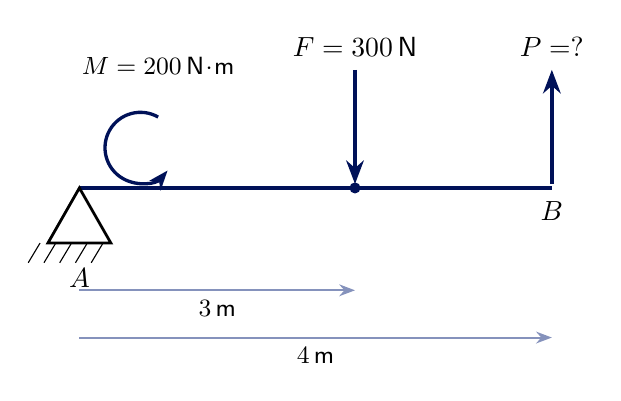
\begin{tikzpicture}
\draw[line width=1.5pt, mainblue] (0,0) -- (6,0);
\draw[line width=1pt] (0,0) -- (-0.4,-0.7) -- (0.4,-0.7) -- cycle;
\foreach \x in {-0.5,-0.3,...,0.3} {\draw[line width=0.4pt] (\x,-0.7) -- (\x-0.15,-0.95);}
\node[below] at (0,-0.9) {$A$};
\node[below] at (6,-0.05) {$B$};

\draw[moment, -{Stealth[length=2.5mm]}] (1.0,0.9) arc (60:320:0.45);
\node at (1.0,1.55) {\small $M=200\,\text{N}\!\cdot\!\text{m}$};

\fill[mainblue] (3.5,0) circle (2pt);
\draw[force] (3.5,1.5) -- (3.5,0.05);
\node[above] at (3.5,1.55) {$F=300\,\text{N}$};

\draw[force] (6,0.05) -- (6,1.5);
\node[above] at (6,1.55) {$P=?$};

\draw[dim] (0,-1.3) -- (3.5,-1.3);
\node[below] at (1.75,-1.3) {\small $3\,\text{m}$};
\draw[dim] (0,-1.9) -- (6,-1.9);
\node[below] at (3,-1.9) {\small $4\,\text{m}$};
\end{tikzpicture}

% ---------- Exercise 2.4: force + couple reduced to a single equivalent force ----------
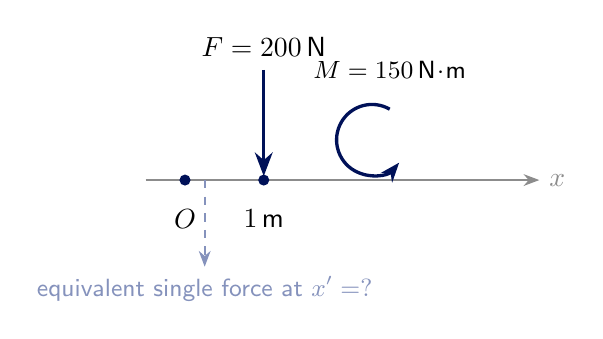
\begin{tikzpicture}
\draw[-{Stealth[length=2mm]}, line width=0.6pt, color=black!45] (-0.5,0) -- (4.5,0) node[right] {$x$};
\fill[mainblue] (0,0) circle (2pt);
\node[below] at (0,-0.25) {$O$};
\fill[mainblue] (1,0) circle (2pt);
\node[below] at (1,-0.25) {$1\,\text{m}$};
\draw[force] (1,1.4) -- (1,0.05);
\node[above] at (1,1.45) {$F=200\,\text{N}$};
\draw[moment, -{Stealth[length=2.5mm]}] (2.6,0.9) arc (60:320:0.45);
\node at (2.6,1.4) {\small $M=150\,\text{N}\!\cdot\!\text{m}$};
\draw[dim, dashed] (0.25,0) -- (0.25,-1.1);
\node[below, color=accent] at (0.25,-1.1) {\small equivalent single force at $x'=?$};
\end{tikzpicture}

\end{document}
